\documentclass[11pt]{article}
\usepackage{amsmath, amssymb, amsfonts}
\usepackage{graphicx}
\usepackage{hyperref}
\usepackage{geometry}
\usepackage{tikz}
\usepackage{xcolor}
\usetikzlibrary{shapes.geometric, arrows.meta, positioning, fit, backgrounds, calc}

\geometry{margin=1in}

% Define colors
\definecolor{inputcolor}{RGB}{200,0,0}
\definecolor{blockcolor}{RGB}{220,220,220}
\definecolor{outputcolor}{RGB}{0,100,200}
\definecolor{learningcolor}{RGB}{100,150,200}
\definecolor{losscolor}{RGB}{220,180,100}
\definecolor{nncolor}{RGB}{255,235,180}
\definecolor{autodiffcolor}{RGB}{180,230,180}

% Define styles
\tikzstyle{block} = [rectangle, draw, fill=blockcolor, text width=3cm, text centered, minimum height=2cm, rounded corners]
\tikzstyle{smallblock} = [rectangle, draw, fill=learningcolor, text width=2.2cm, text centered, minimum height=0.8cm, rounded corners]
\tikzstyle{lossblock} = [rectangle, draw, fill=losscolor, text width=2.2cm, text centered, minimum height=0.8cm, rounded corners]
\tikzstyle{arrow} = [-Stealth, thick]
\tikzstyle{redarrow} = [-Stealth, thick, color=inputcolor]
\tikzstyle{bluearrow} = [-Stealth, thick, color=outputcolor]
\tikzstyle{nnbox} = [rectangle, draw, fill=nncolor, text width=1.8cm, text centered, minimum height=0.8cm, rounded corners]
\tikzstyle{autodiffbox} = [rectangle, draw, fill=autodiffcolor, text width=1.8cm, text centered, minimum height=0.8cm, rounded corners]

\title{Introduction to Closure Problem with Visual Illustrations}
\author{Matthew G. Galarza}
\date{\today}

\begin{document}
\maketitle

\section{Introduction}

A fundamental challenge in the modeling of complex dynamical systems is one of closure where the evolution of the resolved variables depends on unresolved states, processes, and scales that are not directly accessible. This mismatch between the "true" system and its analytical or reduced approximation stems from partial observability, missing or inaccurate physics, and parameter uncertainty. The challenge is ubiquitous, appearing in a variety of diverse fields including turbulence modeling, climate science, molecular dynamics, and biological systems.

\subsection{General Mathematical Formulation}

Consider a general dynamical system with state variables partitioned into resolved (observable) and unresolved (hidden) components:
\begin{equation}
\frac{d}{dt}\begin{bmatrix} \mathbf{u} \\ \mathbf{v} \end{bmatrix} = \begin{bmatrix} f(\mathbf{u}, \mathbf{v}, t) \\ g(\mathbf{u}, \mathbf{v}, t) \end{bmatrix}
\end{equation}
where $\mathbf{u}$ represents resolved/observable states and $\mathbf{v}$ represents unresolved/hidden states. When only $\mathbf{u}$ is observable, the evolution equation becomes:
\begin{equation}
\frac{d\mathbf{u}}{dt} = f(\mathbf{u}, \mathbf{v}, t)
\end{equation}
The closure problem emerges because the right-hand side depends on the unobservable $\mathbf{v}$, requiring a closure model:
\begin{equation}
\frac{d\mathbf{u}}{dt} = f(\mathbf{u}, \mathcal{C}(\mathbf{u}, t), t)
\end{equation}
where $\mathcal{C}(\mathbf{u}, t)$ is the closure approximation that models the effect of unresolved variables.

\subsection{The Observability Gap}

The closure problem is particularly acute when there is a significant disparity between analytical models and experimental measurements. Figure~\ref{fig:observability_gap} illustrates this challenge: while analytical simulations provide access to the full high-dimensional state space $\mathbf{u}(t) \in \mathbb{R}^n$, experimental measurements often yield only a low-dimensional observable $\mathbf{u}(t) \in \mathbb{R}^m$ where $m \ll n$. This observability gap necessitates the development of closure models that can reconstruct or approximate the dynamics of hidden states from limited measurements.

\begin{figure}[h]
\centering
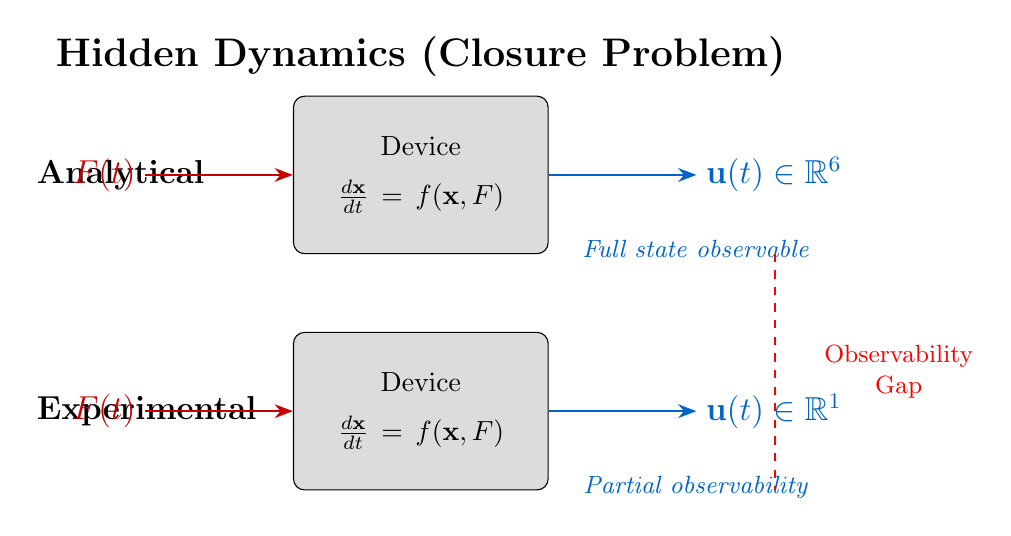
\begin{tikzpicture}[node distance=3cm]
    % Title
    \node[font=\Large\bfseries] at (0, 3) {Hidden Dynamics (Closure Problem)};
    
    % Analytical scenario
    \node[font=\large\bfseries, anchor=west] (anal_label) at (-5, 1.5) {Analytical};
    \node[block] (device1) at (0, 1.5) {Device\\[0.2cm]$\frac{d\mathbf{x}}{dt} = f(\mathbf{x}, F)$};
    \node[font=\large, anchor=east, color=inputcolor] (F1) at (-3.5, 1.5) {$F(t)$};
    \node[font=\large, anchor=west, color=outputcolor] (u1) at (3.5, 1.5) {$\mathbf{u}(t) \in \mathbb{R}^6$};
    \draw[redarrow] (F1) -- (device1);
    \draw[bluearrow] (device1) -- (u1);
    \node[font=\small, anchor=north, color=outputcolor] at (3.5, 0.8) {\textit{Full state observable}};
    
    % Experimental scenario
    \node[font=\large\bfseries, anchor=west] (exp_label) at (-5, -1.5) {Experimental};
    \node[block] (device2) at (0, -1.5) {Device\\[0.2cm]$\frac{d\mathbf{x}}{dt} = f(\mathbf{x}, F)$};
    \node[font=\large, anchor=east, color=inputcolor] (F2) at (-3.5, -1.5) {$F(t)$};
    \node[font=\large, anchor=west, color=outputcolor] (u2) at (3.5, -1.5) {$\mathbf{u}(t) \in \mathbb{R}^1$};
    \draw[redarrow] (F2) -- (device2);
    \draw[bluearrow] (device2) -- (u2);
    \node[font=\small, anchor=north, color=outputcolor] at (3.5, -2.2) {\textit{Partial observability}};
    
    % Annotation showing the gap
    \draw[dashed, thick, color=red] (4.5, 0.5) -- (4.5, -2.5);
    \node[font=\small, color=red, align=center, anchor=west] at (5, -1) {Observability\\Gap};
\end{tikzpicture}
\caption{The observability gap between analytical models and experimental measurements. Analytical simulations provide access to the full state vector, while experiments yield only partial observations, creating the closure problem.}
\label{fig:observability_gap}
\end{figure}

\subsection{Modern Data-Driven Approaches}

\subsubsection{Neural Closure Models}

Recent advances leverage neural networks to learn closure relationships from data:
\begin{equation}
\mathcal{C}(\mathbf{u}, t) = \mathcal{N}_{\boldsymbol{\theta}}(\mathbf{u}, t) + \int_{-\infty}^{t} \mathcal{K}_{\boldsymbol{\phi}}(\mathbf{u}(s), t-s) ds
\end{equation}
where $\mathcal{N}_{\boldsymbol{\theta}}$ captures Markovian (instantaneous) effects and $\mathcal{K}_{\boldsymbol{\phi}}$ models non-Markovian (memory) effects.

Two paradigms for learning closure models are illustrated in Figure~\ref{fig:learning_paradigms}: \textit{a-priori} learning, where closure parameters are determined before model reduction, and \textit{a-posteriori} learning, where closure is learned directly in the reduced space using observed data. The a-posteriori approach is particularly relevant when full-state observations are unavailable.

\begin{figure}[h]
\centering
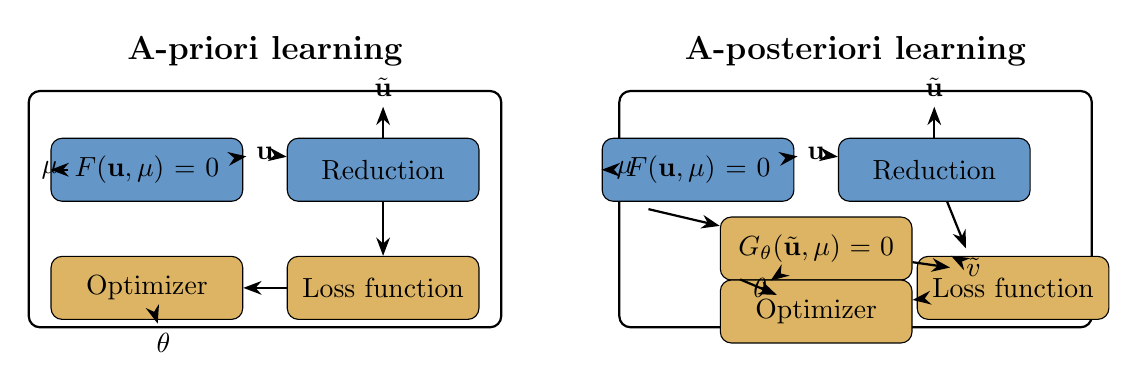
\begin{tikzpicture}[node distance=1.5cm and 2cm]
    % A-priori learning
    \node[font=\large\bfseries] (apriori_title) at (-3.5, 3) {A-priori learning};
    \draw[rounded corners, thick] (-6.5, 2.5) rectangle (-0.5, -0.5);
    
    \node[smallblock] (F1) at (-5, 1.5) {$F(\mathbf{u}, \mu) = 0$};
    \node[smallblock] (R1) at (-2, 1.5) {Reduction};
    \node[lossblock] (L1) at (-2, 0) {Loss function};
    \node[lossblock] (O1) at (-5, 0) {Optimizer};
    
    \node[font=\normalsize, anchor=east] (mu1) at (-6, 1.5) {$\mu$};
    \node[font=\normalsize, anchor=south] (u1) at (-3.5, 1.5) {$\mathbf{u}$};
    \node[font=\normalsize, anchor=south] (utilde1) at (-2, 2.3) {$\tilde{\mathbf{u}}$};
    \node[font=\normalsize, anchor=west] (theta1) at (-5, -0.7) {$\theta$};
    
    \draw[arrow] (mu1) -- (F1);
    \draw[arrow] (F1) -- (u1);
    \draw[arrow] (u1) -- (R1);
    \draw[arrow] (R1) -- (utilde1);
    \draw[arrow] (R1) -- (L1);
    \draw[arrow] (L1) -- (O1);
    \draw[arrow] (O1) -- (theta1);
    
    % A-posteriori learning
    \node[font=\large\bfseries] (aposteriori_title) at (4, 3) {A-posteriori learning};
    \draw[rounded corners, thick] (1, 2.5) rectangle (7, -0.5);
    
    \node[smallblock] (F2) at (2, 1.5) {$F(\mathbf{u}, \mu) = 0$};
    \node[smallblock] (R2) at (5, 1.5) {Reduction};
    \node[lossblock] (G2) at (3.5, 0.5) {$G_{\theta}(\tilde{\mathbf{u}}, \mu) = 0$};
    \node[lossblock] (L2) at (6, 0) {Loss function};
    \node[lossblock] (O2) at (3.5, -0.3) {Optimizer};
    
    \node[font=\normalsize, anchor=east] (mu2) at (1.3, 1.5) {$\mu$};
    \node[font=\normalsize, anchor=south] (u2) at (3.5, 1.5) {$\mathbf{u}$};
    \node[font=\normalsize, anchor=south] (utilde2) at (5, 2.3) {$\tilde{\mathbf{u}}$};
    \node[font=\normalsize, anchor=north] (v2) at (5.5, 0.5) {$\tilde{v}$};
    \node[font=\normalsize, anchor=east] (theta2) at (3, 0) {$\theta$};
    
    \draw[arrow] (mu2) -- (F2);
    \draw[arrow] (F2) -- (u2);
    \draw[arrow] (u2) -- (R2);
    \draw[arrow] (R2) -- (utilde2);
    \draw[arrow] (R2) -- (v2);
    \draw[arrow] (v2) -- (L2);
    \draw[arrow] ($(mu2) + (0.3, -0.5)$) -- (G2);
    \draw[arrow] (G2) -- ($(v2) + (-0.3, 0)$);
    \draw[arrow] (L2) -- (O2);
    \draw[arrow] (O2) -- (theta2);
    \draw[arrow] (theta2) -- (G2);
    
\end{tikzpicture}
\caption{Learning paradigms for closure models. \textbf{A-priori learning}: Parameters are learned from full-state simulations before reduction. \textbf{A-posteriori learning}: Closure is learned directly in the reduced space using the learned model $G_{\theta}$ to approximate unresolved dynamics.}
\label{fig:learning_paradigms}
\end{figure}

\subsubsection{Physics-Informed Machine Learning}

Hybrid approaches combine physical constraints with data-driven learning:
\begin{itemize}
    \item \textbf{Universal Differential Equations}: Augment known physics with neural network corrections
    \item \textbf{Neural Differential-Algebraic Equations}: Enforce conservation laws through algebraic constraints
    \item \textbf{Operator learning}: Learn mappings between function spaces for closure relationships
\end{itemize}

A critical distinction in physics-informed approaches is between \textit{soft constraints}, which penalize violations in the loss function, and \textit{hard constraints}, which enforce physical laws by construction. Figure~\ref{fig:constraint_approaches} illustrates this difference: soft constraints minimize violations through regularization (e.g., $\|\frac{\partial u}{\partial x} + \frac{\partial v}{\partial y}\|^2$), while hard constraints ensure exact satisfaction through architectural design.

\begin{figure}[h]
\centering
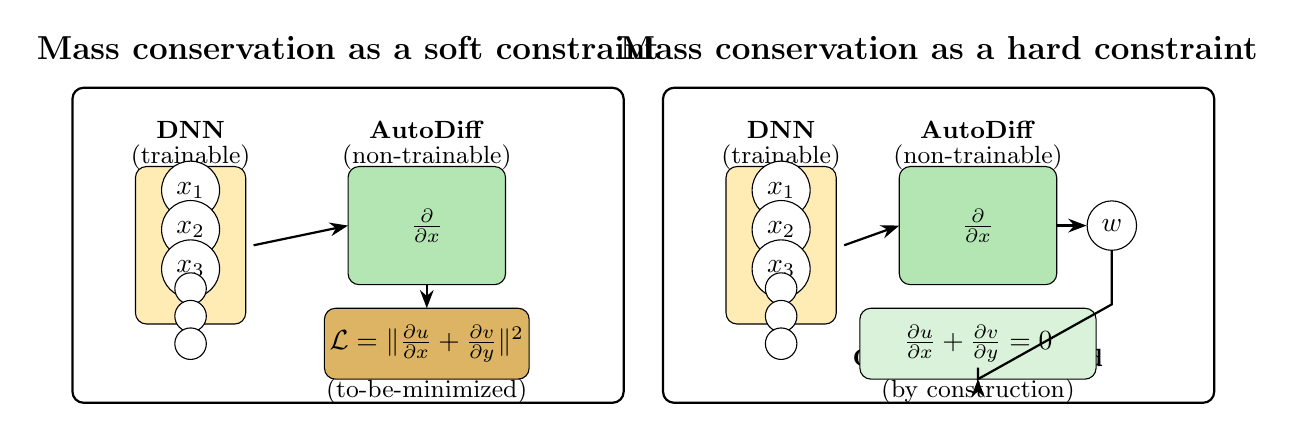
\begin{tikzpicture}[node distance=1.2cm and 1.5cm]
    % Soft constraint
    \node[font=\large\bfseries] (soft_title) at (-3.5, 3.5) {Mass conservation as a soft constraint};
    \draw[rounded corners, thick] (-7, 3) rectangle (0, -1);
    
    % Neural network representation
    \node[font=\small, anchor=north] at (-5.5, 2.7) {\textbf{DNN}};
    \node[font=\small, anchor=north] at (-5.5, 2.4) {(trainable)};
    \draw[rounded corners, fill=nncolor, draw=black] (-6.2, 2) rectangle (-4.8, 0);
    
    % Network nodes
    \foreach \i in {1,2,3} {
        \node[circle, draw, fill=white, minimum size=0.4cm] (input\i) at (-5.5, {2.2 - 0.5*\i}) {$x_{\i}$};
    }
    \foreach \i in {1,2,3} {
        \node[circle, draw, fill=white, minimum size=0.4cm] (hidden\i) at (-5.5, {0.8 - 0.35*\i}) {};
    }
    
    \node[font=\small, anchor=north] at (-2.5, 2.7) {\textbf{AutoDiff}};
    \node[font=\small, anchor=north] at (-2.5, 2.4) {(non-trainable)};
    \draw[rounded corners, fill=autodiffcolor, draw=black] (-3.5, 2) rectangle (-1.5, 0.5);
    \node[font=\normalsize] at (-2.5, 1.25) {$\frac{\partial}{\partial x}$};
    
    \draw[arrow] (-4.7, 1) -- (-3.5, 1.25);
    
    \node[font=\small, anchor=north, align=center] at (-2.5, -0.2) {\textbf{Loss term}\\(to-be-minimized)};
    \draw[rounded corners, fill=losscolor, draw=black] (-3.8, 0.2) rectangle (-1.2, -0.7);
    \node[font=\normalsize] at (-2.5, -0.25) {$\mathcal{L} = \|\frac{\partial u}{\partial x} + \frac{\partial v}{\partial y}\|^2$};
    
    \draw[arrow] (-2.5, 0.5) -- (-2.5, 0.2);
    
    % Hard constraint
    \node[font=\large\bfseries] (hard_title) at (4, 3.5) {Mass conservation as a hard constraint};
    \draw[rounded corners, thick] (0.5, 3) rectangle (7.5, -1);
    
    % Neural network representation
    \node[font=\small, anchor=north] at (2, 2.7) {\textbf{DNN}};
    \node[font=\small, anchor=north] at (2, 2.4) {(trainable)};
    \draw[rounded corners, fill=nncolor, draw=black] (1.3, 2) rectangle (2.7, 0);
    
    % Network nodes
    \foreach \i in {1,2,3} {
        \node[circle, draw, fill=white, minimum size=0.4cm] (input2\i) at (2, {2.2 - 0.5*\i}) {$x_{\i}$};
    }
    \foreach \i in {1,2,3} {
        \node[circle, draw, fill=white, minimum size=0.4cm] (hidden2\i) at (2, {0.8 - 0.35*\i}) {};
    }
    
    \node[font=\small, anchor=north] at (4.5, 2.7) {\textbf{AutoDiff}};
    \node[font=\small, anchor=north] at (4.5, 2.4) {(non-trainable)};
    \draw[rounded corners, fill=autodiffcolor, draw=black] (3.5, 2) rectangle (5.5, 0.5);
    \node[font=\normalsize] at (4.5, 1.25) {$\frac{\partial}{\partial x}$};
    
    \node[circle, draw, fill=white, minimum size=0.5cm] (w) at (6.2, 1.25) {$w$};
    
    \draw[arrow] (2.8, 1) -- (3.5, 1.25);
    \draw[arrow] (5.5, 1.25) -- (w);
    
    \node[font=\small, anchor=north, align=center] at (4.5, -0.2) {\textbf{Constraint satisfied}\\(by construction)};
    \draw[rounded corners, fill=autodiffcolor!50, draw=black] (3, 0.2) rectangle (6, -0.7);
    \node[font=\normalsize] at (4.5, -0.25) {$\frac{\partial u}{\partial x} + \frac{\partial v}{\partial y} = 0$};
    
    \draw[arrow] (w) -- ($(w) + (0, -1)$) -- (4.5, -0.7) -- (4.5, -0.7);
    
\end{tikzpicture}
\caption{Constraint enforcement strategies. \textbf{Soft constraints} (left): Physical laws are incorporated as penalty terms in the loss function, minimized during training. \textbf{Hard constraints} (right): Physical laws are enforced exactly through architectural design, guaranteeing satisfaction by construction.}
\label{fig:constraint_approaches}
\end{figure}

\subsection{Key Challenges in Closure Modeling}

\begin{enumerate}
    \item \textbf{Structural uncertainty}: The functional form of the closure is often unknown
    \item \textbf{Scale separation}: Unresolved scales may span multiple orders of magnitude
    \item \textbf{Non-Markovian effects}: Hidden states may have long memory effects
    \item \textbf{Generalization}: Closure models must extrapolate to conditions beyond training data
    \item \textbf{Stability}: Inappropriate closures can lead to numerical instabilities or unphysical solutions
    \item \textbf{Interpretability}: Understanding what the closure model has learned remains challenging
\end{enumerate}

These challenges motivate the systematic investigation of various closure modeling approaches, from classical state estimation techniques to modern neural architectures, which form the focus of this research.

\end{document}